\section{Pruebas.}
\label{sec:pruebas}

\subsection{Pruebas de usabilidad.}

La evaluación de usabilidad del launcher se realizó mediante una encuesta a estudiantes universitarios, grupo objetivo de la aplicación. Los participantes, jóvenes adultos entre 22 y 25 años que usan su smartphone regularmente, reflejan el perfil típico de usuarios que buscan mejorar su concentración y productividad. La mayoría manifestó ser consciente del tiempo excesivo que pasa en su smartphone, especialmente en momentos inapropiados como durante actividades académicas o de descanso, y expresó interés en herramientas que les ayuden a regular este uso.

Cabe destacar que el número de encuestados fue reducido debido a las particularidades técnicas y éticas del proyecto. Dado que se trata de una aplicación para Android que se debe instalar, no es posible su despliegue en un entorno web ni su distribución pública, ya que su instalación requiere permisos especiales relacionados con acceso a información del sistema operativo y el monitoreo del tiempo de uso de las aplicaciones, aspectos que son sensibles en términos de privacidad.

Por estas razones, se decidió aplicar la encuesta únicamente a un grupo selecto de usuarios que aceptaron instalar la aplicación en sus dispositivos personales y participar bajo las condiciones previamente informadas, garantizando así un entorno de prueba controlado, seguro y éticamente responsable.

La Figura \ref{fig:interfaz_intuitiva} muestra que la mayoría de los participantes considera que el launcher es intuitivo y fácil de usar. El 71,4\% de los participantes calificó con la puntuación máxima (5) la intuición de la interfaz del launcher, mientras que el 28,6\% le otorgó una calificación de 4.

\begin{figure}[h]
  \caption{Primera prueba de usabilidad.}
  \label{fig:interfaz_intuitiva}
  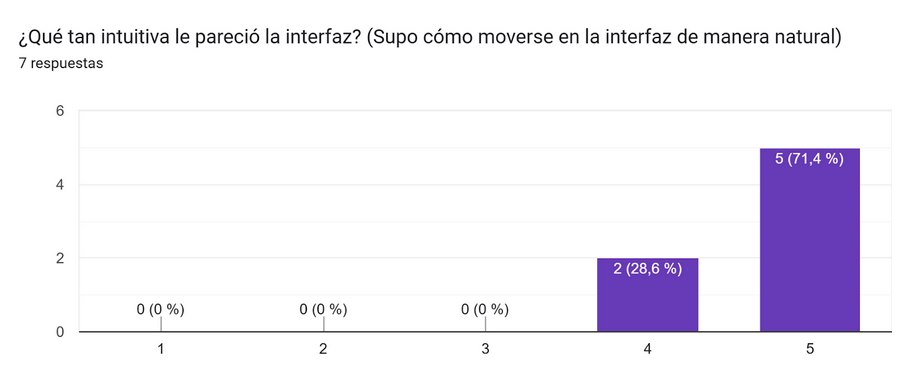
\includegraphics[width=\textwidth]{Figuras/interfaz_intuitiva.png}
  \centering
\end{figure}

En relación con la apariencia de la aplicación, los resultados presentes en la Figura \ref{fig:interfaz_agradable} reflejan una alta aceptación del diseño minimalista, funcional y centrado en la productividad por parte de los usuarios. El 71,4\% de los encuestados calificó el diseño de la interfaz con la puntuación máxima (5), mientras que el 28,6\% otorgó una calificación de 4.

\begin{figure}[h]
  \caption{Segunda prueba de usabilidad.}
  \label{fig:interfaz_agradable}
  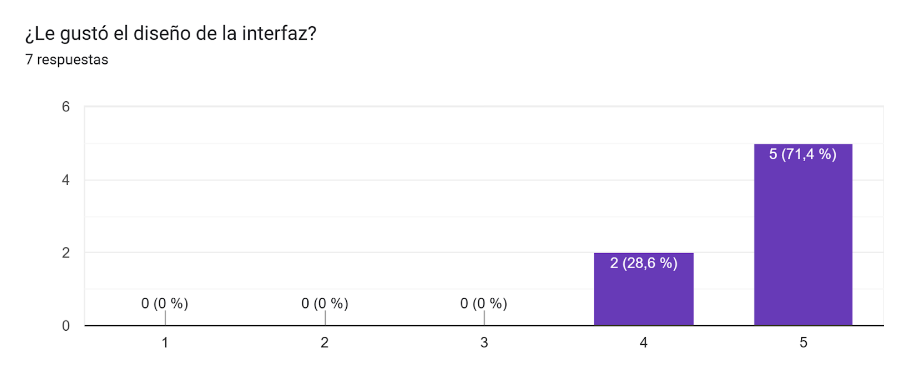
\includegraphics[width=\textwidth]{Figuras/interfaz_agradable.png}
  \centering
\end{figure}

Los resultados de la tercera prueba de usabilidad, mostrados en la Figura \ref{fig:mejores_caracteristicas}, indican que el diseño minimalista fue identificado como la característica más útil del launcher por el 100\% de los participantes. En segundo lugar, se destacan la gestión de tareas y hábitos (71,4\%) y el límite de uso de aplicaciones (71,4\%), dos de las principales funcionalidades del launcher. 

\begin{figure}[h]
  \caption{Tercera prueba de usabilidad.}
  \label{fig:mejores_caracteristicas}
  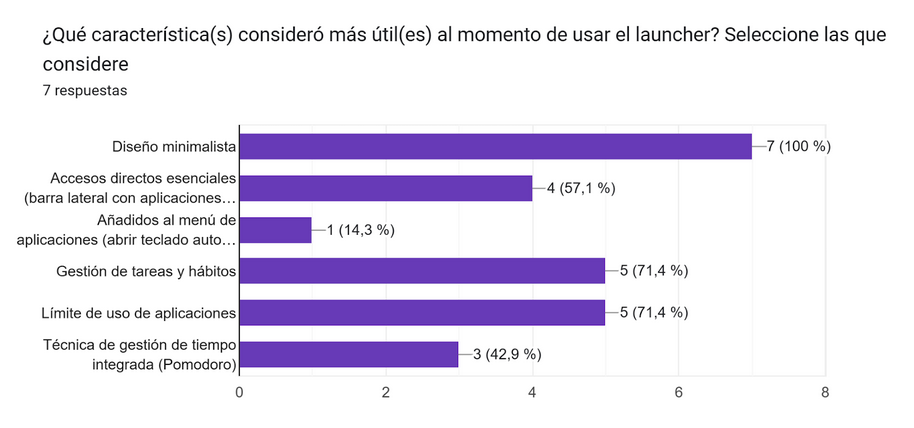
\includegraphics[width=\textwidth]{Figuras/mejores_caracteristicas.png}
  \centering
\end{figure}

El 100\% de los encuestados, según la Figura \ref{fig:cumplio_objetivo}, coincidió en que el launcher cumplió con su objetivo de proporcionar una interfaz de pantalla de inicio minimalista, funcional y con herramientas que pueden ayudar a evitar las distracciones en el uso del Smartphone y ayudar a mejorar la productividad durante el periodo en que fue utilizado.

\begin{figure}[h]
  \caption{Cuarta prueba de usabilidad.}
  \label{fig:cumplio_objetivo}
  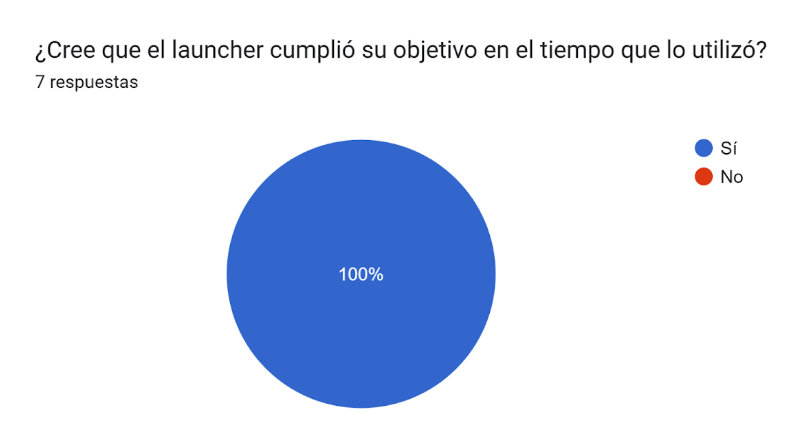
\includegraphics[width=\textwidth]{Figuras/cumplio_objetivo.png}
  \centering
\end{figure}

En respuesta a la pregunta: \textbf{¿Qué fue lo que más le gustó de la aplicación?}, se destacan la funcionalidad de gestión de tareas y hábitos, la practicidad general de la aplicación y su diseño minimalista. También se resaltó el hecho de que las tareas se visualizan de inmediato al iniciar el launcher para mantener el enfoque en las metas personales.

\begin{figure}[h]
  \caption{Quinta prueba de usabilidad.}
  \label{fig:mas_valorado}
  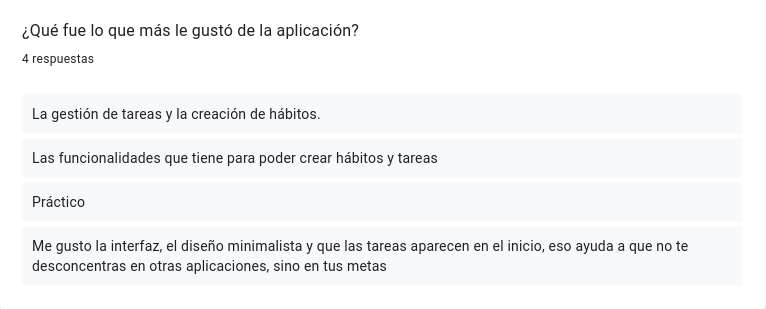
\includegraphics[width=0.92\textwidth]{Figuras/mas_valorado.png}
  \centering
\end{figure}

En cuanto a la pregunta: \textbf{¿Qué fue lo que menos le gustó de la aplicación, qué errores experimentó o en qué podría mejorar?}, los participantes mencionaron principalmente la falta de opciones de personalización, problemas de rendimiento al iniciar la aplicación o al abrir el teclado al entrar al menú de aplicaciones. Por otro lado, uno de los encuestados destacó que la aplicación funcionó sin inconvenientes, lo cual sugiere que la experiencia puede variar según el dispositivo o la configuración.

\begin{figure}[h]
  \caption{Sexta prueba de usabilidad.}
  \label{fig:oportunidades_mejora}
  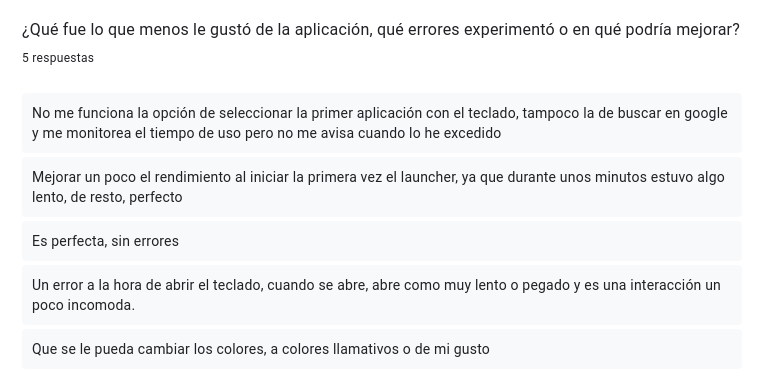
\includegraphics[width=0.92\textwidth]{Figuras/oportunidades_mejora.png}
  \centering
\end{figure}

En respuesta a: \textbf{¿Qué características cree que se podrían añadir que ayuden a cumplir mejor el objetivo de la aplicación?}, los participantes sugirieron una barra de desplazamiento para buscar por orden alfabético las aplicaciones, la posibilidad de bloquear aplicaciones independientemente de si tienen o no límite de tiempo y características de monitoreo de salud, como seguimiento del sueño.

\begin{figure}[h]
  \caption{Séptima prueba de usabilidad.}
  \label{fig:caracteristicas_adicionales}
  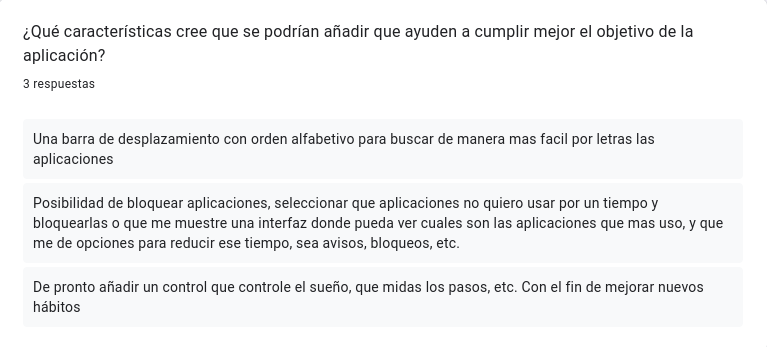
\includegraphics[width=0.92\textwidth]{Figuras/caracteristicas_adicionales.png}
  \centering
\end{figure}

Por último, en la pregunta: \textbf{¿Consideraría seguir usando este Launcher o uno con un enfoque similar en su día a día?}, el 71,4\% de los participantes manifestó su intención de seguir utilizando el launcher o una herramienta con un enfoque similar en su rutina diaria. Por otro lado, el 28,6\% indicó que "tal vez" lo haría, lo cual, aunque no representa una afirmación definitiva, demuestra una disposición positiva hacia la aplicación.

\begin{figure}[h]
  \caption{Octava prueba de usabilidad.}
  \label{fig:continuar_usando}
  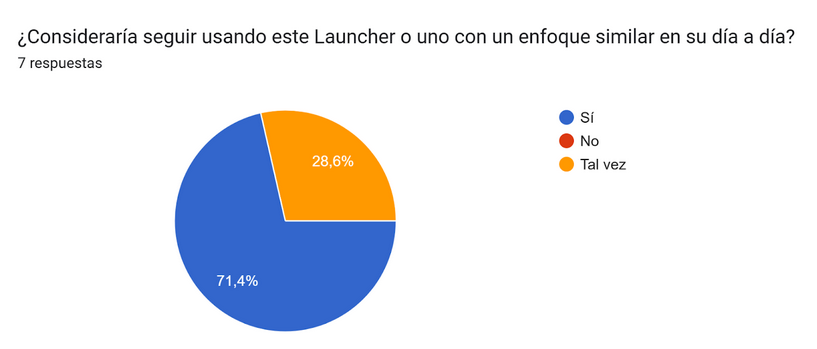
\includegraphics[width=0.92\textwidth]{Figuras/continuar_usando.png}
  \centering
\end{figure}